\chapter{Proper Time, Local Flatness, and Curvature from Parallel Transport}

The lecture begins by announcing two long-range goals: to say more about geodesics, and to connect geodesics more directly with gravity. But it does not move there immediately. First the space-time metric has to be rebuilt, because without proper time, signature, and covariant differentiation already in hand, the later discussion of curvature would float free of its physical meaning. Only after that reset does the lecture choose, after a brief hesitation, to take up curvature first. The result is a chapter whose logic is quite deliberate: proper time, then the distinction between curved coordinates and genuine curvature, then local flatness, then geodesics and parallel transport, and only then curvature as the failure of parallel transport to be path-independent.

\section{Space-Time Metric, Proper Time, and the Minkowski Signature}

For the first part of the lecture we are asked to think about space-time rather than space alone. The mathematical machinery is the same as before, but the notation shifts. Instead of the spatial indices \(m,n,\ldots\), Susskind now uses Greek indices \(\mu,\nu,\ldots\), running over \(0,1,2,3\), with \(0\) the time direction and \(1,2,3\) the spatial directions.

There is, again, a metric, and therefore a notion of interval. In space-time the interval is written as proper time:
\begin{align}
d\tau^{2} &= g_{\mu\nu}\,dx^{\mu}dx^{\nu}, \\
\eta_{\mu\nu} &=
\begin{pmatrix}
1 & 0 & 0 & 0 \\
0 & -1 & 0 & 0 \\
0 & 0 & -1 & 0 \\
0 & 0 & 0 & -1
\end{pmatrix}.
\end{align}
Here \(\eta_{\mu\nu}\) is the special-relativistic metric, constant everywhere, and the lecture uses the signature \((+---)\): one plus sign for the time direction and three minus signs for the spatial ones.

Strictly speaking, one should not say that the metric simply \emph{is} this matrix once and for all. The metric is a tensor. What is true is that in these coordinates its components take this form. That is exactly why the lecture pauses over the point that the metric tensor is a tensor, even in this simplest case.

\begin{figure}[h]
\centering

\includegraphics[width=0.62\textwidth]{lecture_06_figure_02.png}
\caption{Minkowski metric and the proper-time interval, written on the board from top to bottom as general contraction, explicit matrix, and component form.}
\end{figure}

The last line on the board is slightly cramped, but the intended formula is clear from the lecture:
\begin{equation}
d\tau^{2} = dt^{2} - \frac{dx^{2}+dy^{2}+dz^{2}}{c^{2}}.
\end{equation}
If we choose units with \(c=1\), this reduces to
\begin{equation}
d\tau^{2} = dt^{2} - dx^{2} - dy^{2} - dz^{2}.
\end{equation}
The infinitesimal displacement \(dx^{\mu}\) is the little step along the worldline, and \(d\tau\) is the corresponding interval measured along that worldline.

The lecture also pauses over the phrase that the speed of light is ``large.'' Of course \(c\) is neither large nor small in itself. What is meant is that the speeds of the objects we care about are small compared with \(c\). Under those circumstances the spatial correction is negligible, and so
\begin{equation}
d\tau \approx dt
\end{equation}
for slow motion. But that is only an approximation. In general the proper time along the trajectory is not the same thing as the coordinate time of a chosen frame.

\subsection{Question \& Answer}

\paragraph{Why does the moving clock record \(d\tau\) rather than \(dt\)?}

Because the clock moves with the object. It does not measure the time coordinate of some externally chosen system of coordinates; it measures the interval along the object's own worldline. The lecture makes the point with a geometric analogy: a tape measure laid along a curve in space does not record \(x\) or \(y\), it records the distance \emph{along the curve}. In the same spirit, the moving clock is a kind of space-time tape measure. It marks off proper time along the trajectory itself. Coordinate time \(dt\) belongs to a coordinate system; proper time \(d\tau\) belongs to the motion.

\section{Curved Coordinates Are Not Yet Curvature}

With the interval and proper time back in place, the lecture makes the bridge to general relativity by analogy. Flat space is to curved space as special relativity is to curved space-time. The formal tools are the same: metric, tensors, Christoffel symbols, covariant derivatives. What changes is that the metric need no longer be constant, and therefore the geometry itself may be nontrivial.

But there is a distinction the lecture is determined not to lose. Curved coordinates are not yet the same thing as genuine curvature.

In flat space or flat space-time one does not ordinarily need curvilinear coordinates at all. If our only goal were to make life easy, introducing them would seem perverse. We introduce them because accelerated frames are physically important. In an inertial frame objects move on straight lines; in an accelerated frame the same motions look curved, and the coordinate lines themselves are bent.

\begin{figure}[h]
\centering
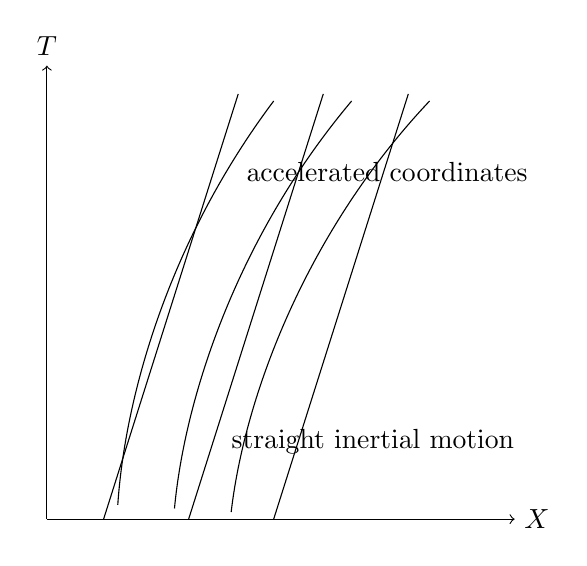
\begin{tikzpicture}[scale=0.9]
\draw[->] (0,0) -- (6.6,0) node[right] {$X$};
\draw[->] (0,0) -- (0,6.4) node[above] {$T$};

\draw (0.8,0) -- (2.7,6.0);
\draw (2.0,0) -- (3.9,6.0);
\draw (3.2,0) -- (5.1,6.0);

\draw (1.0,0.2) .. controls (1.1,1.7) and (1.7,3.9) .. (3.2,5.9);
\draw (1.8,0.15) .. controls (1.95,1.75) and (2.7,4.0) .. (4.3,5.9);
\draw (2.6,0.1) .. controls (2.8,1.8) and (3.7,4.1) .. (5.4,5.9);

\node at (4.8,4.9) {accelerated coordinates};
\node at (4.6,1.1) {straight inertial motion};
\end{tikzpicture}
\caption{A schematic Minkowski diagram: straight inertial trajectories in \((T,X)\), together with a curved coordinate family adapted to accelerated motion.}
\end{figure}

This is the old elevator story. An accelerated coordinate system can imitate a gravitational field. That is the content of the equivalence principle in its local form. Had Einstein not taken acceleration and gravity seriously together, nobody would have volunteered curved coordinates in otherwise flat physics.

But this imitation is only local. A fake gravitational field produced by acceleration can be removed by changing coordinates again. A real gravitational field cannot be removed everywhere in that way.

The lecture's example is a star pulling an elevator toward it. If the elevator is small and allowed to fall freely, experiments inside it look inertial. That is the local victory of free fall. But the victory is not complete. The field varies slightly across the elevator, and so tidal forces remain. One side of the elevator wants to fall differently from another. That residual variation is the first sign that something genuine is present. It is the obstruction to removing the gravitational field globally.

At this point, after a brief hesitation and even a vote in the room, the lecture decides to do curvature before returning to geodesics. That is the right order for the story. Before we can say how things move in curved space-time, we must first say what it means for the geometry itself to be flat or curved.

\section{What Does It Mean for Space or Space-Time to Be Flat?}

Now the discussion shifts back to ordinary geometric notation, with Latin indices \(m,n,r,s,\ldots\). The first question is the obvious one: what does it mean for a space, or a space-time, to be flat?

The answer is not that every coordinate system looks Cartesian. The answer is that one \emph{can find} coordinates in which the metric is constant. In the simplest Euclidean case one may choose coordinates with
\[
g_{mn}=\delta_{mn},
\]
but the lecture immediately points out that even this is stronger than necessary. If the coordinate axes are straight and uniformly spaced but not mutually perpendicular, the metric will not be \(\delta_{mn}\), yet it will still be constant from point to point. So the real definition is constancy, not orthonormality.

To put it slightly differently, a geometry is flat if one can choose coordinates so that the derivatives of the metric vanish:
\begin{equation}
\partial_{s}g_{mn}=0.
\end{equation}
This is already a three-index object, with \(m\) and \(n\) symmetric. In a truly flat geometry one can make all such derivatives vanish everywhere.

The lecture then turns the statement local. Even without having defined curvature formally, one can already assert that at a \emph{single point} it is always possible to choose coordinates so that the first derivatives of the metric vanish there. That is the mathematical counterpart of the freely falling elevator. One can always flatten the geometry locally. What curvature will measure is the obstruction to doing this everywhere at once.

There is also an implicit regularity assumption here. The lecture says it plainly when a student asks about wildly wiggly metrics. We assume the metric is continuous and differentiable, at least in the region under discussion. There can be exceptions, and those exceptions are genuine singularities. But one must not confuse a singular coordinate system with a singular geometry. Polar coordinates are bad at the origin, yet the plane itself is perfectly smooth there. A true singularity is a place where no coordinate system makes the metric smooth. The cone tip will supply the example.

\section{Local Coordinate Freedom and Vanishing First Derivatives}

The local flattening argument is one of the lecture's technical centers. We begin with coordinates \(x^{m}\) in which the metric is not locally constant at the chosen point. We now look for new coordinates \(y^{m}\) with the same origin and write a local expansion
\begin{equation}
y^{m}=x^{m}+c^{m}{}_{rs}\,x^{r}x^{s}+\cdots.
\end{equation}
The linear term has been chosen to be the identity simply to keep the discussion focused. The real freedom lies in the quadratic coefficients \(c^{m}{}_{rs}\). These are the knobs we adjust in order to influence the first derivatives of the transformed metric.

\begin{figure}[h]
\centering

\includegraphics[width=0.62\textwidth]{lecture_06_figure_04.png}
\caption{The board layout makes the argument visual: the quadratic coordinate freedom sits above, and the target condition on the first derivatives of the metric sits below.}
\end{figure}

The condition we want is
\begin{equation}
\frac{\partial g_{mn}(y)}{\partial y^{s}}=0
\end{equation}
at the chosen point. Why should this be possible? The lecture answers not by performing the full transformation, but by counting equations and unknowns.

First, the coefficients \(c^{m}{}_{rs}\) may be taken symmetric in \(r\) and \(s\):
\begin{equation}
c^{m}{}_{rs}=c^{m}{}_{sr},
\end{equation}
since \(x^{r}x^{s}=x^{s}x^{r}\). For fixed \(m\), that means \(c^{m}{}_{rs}\) is a symmetric \(D\times D\) matrix, and therefore has
\begin{equation}
\frac{D(D+1)}{2}
\end{equation}
independent entries. In three dimensions that gives \(6\), which is exactly the arithmetic checked aloud in the lecture.

\paragraph{Worked derivation.}
\begin{enumerate}
\item For fixed \(m\), the coefficients \(c^{m}{}_{rs}\) form a symmetric matrix in the indices \(r,s\).
\item A symmetric \(D\times D\) matrix has \(D(D+1)/2\) independent entries.
\item Since \(m\) itself runs over \(D\) values, the total number of independent quadratic coefficients is
\begin{equation}
D\cdot \frac{D(D+1)}{2}=\frac{D^{2}(D+1)}{2}.
\end{equation}
\item The object \(\partial_{s}g_{mn}\) also has three indices, with \(m,n\) symmetric.
\item Therefore the number of first-derivative conditions matches the number of adjustable quadratic coefficients.
\item So there is just enough local coordinate freedom to choose coordinates in which all first derivatives of the metric vanish at the selected point.
\end{enumerate}

This is deliberately a local statement. The lecture is explicit that the same counting does not continue indefinitely. Once one asks to eliminate second derivatives, third derivatives, and so on, there are simply too many independent conditions. Thus one can always kill the first derivatives at a point, but in general not the higher derivatives. That is precisely why the higher-order structure contains real geometry.

\subsection{Question \& Answer}

\paragraph{Why is there enough coordinate freedom to kill the first derivatives, but not all higher derivatives?}

Because the quadratic part of the coordinate transformation carries exactly the same index structure as the first derivative of the metric: a three-index object with two symmetric slots. That makes the counting come out exactly right at first order. But higher derivatives bring in more independent components than the available coordinate freedom can absorb. So the lecture's conclusion is not that a curved geometry can be made flat, but only that every geometry can be made \emph{locally} flat through first order at a point.

\section{Christoffel Symbols and Metric Compatibility}

Once the first derivatives of the metric have been set to zero at a point, the next step follows at once. The Christoffel symbols are built from those first derivatives:
\begin{equation}
\Gamma^{r}{}_{mn}
=
\frac{1}{2}g^{rs}\left(
\frac{\partial g_{sm}}{\partial x^{n}}
+
\frac{\partial g_{sn}}{\partial x^{m}}
-
\frac{\partial g_{mn}}{\partial x^{s}}
\right).
\end{equation}
So if
\begin{equation}
\frac{\partial g_{mn}(x)}{\partial x^{r}}=0
\end{equation}
at the point under discussion, then immediately
\begin{equation}
\Gamma^{r}{}_{mn}=0
\end{equation}
there as well.

\begin{figure}[h]
\centering

\includegraphics[width=0.62\textwidth]{lecture_06_figure_05.png}
\caption{The board now turns the counting argument into a geometric statement: vanishing first derivatives imply vanishing Christoffel symbols at the chosen point.}
\end{figure}

This observation already carries one important lesson. Christoffel symbols cannot be tensors. A true tensor that is nonzero somewhere cannot be made to vanish at a point merely by changing coordinates, but the Christoffel symbols can. The lecture says this explicitly: the ability to transform them away at a point is itself evidence that they are not tensorial objects.

The next move is the familiar one:
\begin{equation}
\nabla_{r}g_{mn}=0.
\end{equation}
In components, the covariant derivative of the metric takes the form
\begin{equation}
\nabla_{r}g_{mn}
=
\partial_{r}g_{mn}
-\Gamma^{s}{}_{rm}g_{sn}
-\Gamma^{s}{}_{rn}g_{ms}.
\end{equation}
At the chosen point, in the locally flattened coordinates, the ordinary derivative term vanishes and the Christoffel terms vanish as well. Hence \(\nabla g=0\) there. But \(\nabla g\) is a tensor. If a tensor vanishes in one coordinate system at a point, it vanishes in every coordinate system at that point. Since the point was arbitrary, the standard conclusion is that the metric is covariantly constant everywhere.

This is also the place where the lecture reiterates the original purpose of the covariant derivative. The ordinary derivative of a tensor is not a tensor. The Christoffel symbols are not tensors. But the right combination of the two produces an object that really is tensorial.

\subsection{Question \& Answer}

\paragraph{Is the argument for \(\nabla g=0\) circular?}

A student raises exactly that objection, and Susskind grants the point in part. The argument is a little circular. What it really establishes is the consistency of the standard construction. One assumes the usual Christoffel symbols built from the metric, defines covariant differentiation in the usual way, and then checks that with those definitions the metric is covariantly constant. That is not presented as an immaculate theorem from nowhere. It is presented as the standard, internally consistent choice, and the notes should keep that modest register.

\section{Covariant Derivative Along a Curve, Geodesics, and Parallel Transport}

Only after this detour through local coordinates does the lecture return to the first topic it announced at the beginning: curves. The starting point is the covariant derivative of a vector field \(v^{m}\) along a curve \(x^{m}(s)\). Here \(s\) is simply a parameter along the curve; in the lecture it is thought of as distance along the curve, but the essential formulas do not depend on the special choice of parameter.

The tangent vector is
\begin{equation}
t^{p}=\frac{dx^{p}}{ds},
\end{equation}
and the covariant derivative of \(v^{m}\) along the curve is
\begin{equation}
\frac{D v^{m}}{Ds}
=
\frac{dv^{m}}{ds}
+
\Gamma^{m}{}_{np}\,v^{n}\frac{dx^{p}}{ds}.
\end{equation}
The first term by itself is not tensorial, because the coordinate axes can vary from point to point. The Christoffel term corrects for that change.

A geodesic is now recovered as a special case. We set the vector equal to the tangent vector itself,
\[
v^{m}=\frac{dx^{m}}{ds},
\]
and demand that this tangent vector be parallel transported along the curve:
\begin{equation}
\frac{D}{Ds}\left(\frac{dx^{m}}{ds}\right)=0.
\end{equation}
Then
\begin{equation}
\frac{d^{2}x^{m}}{ds^{2}}
+
\Gamma^{m}{}_{np}\frac{dx^{n}}{ds}\frac{dx^{p}}{ds}
=0.
\end{equation}
This is the geodesic equation in the form used throughout the lecture. A geodesic is the straightest possible curve in the geometry. In flat space it is an ordinary straight line; on a sphere it is a great circle; in a general curved geometry it is whatever path results from going incrementally straight ahead.

But the lecture does not linger there. It immediately widens the discussion. Parallel transport applies to any vector, not only to tangent vectors and not only along geodesics. If a vector \(v^{m}\) along a chosen curve satisfies
\begin{equation}
\frac{D v^{m}}{Ds}=0,
\end{equation}
then we say that \(v^{m}\) is parallel transported along that curve. In words, this is as close as one can come, in a curved geometry or a curved coordinate system, to saying that the vector is constant.

The lecture then rewrites the condition in incremental form. Multiplying by \(ds\), we obtain
\begin{equation}
dv^{m}=-\Gamma^{m}{}_{np}\,v^{n}\,dx^{p}.
\end{equation}
This is the useful update rule. Once the vector is known at one point, together with the Christoffel symbols and the infinitesimal displacement \(dx^{p}\), it tells us how to advance the vector to the neighboring point so that the covariant derivative continues to vanish.

\paragraph{Worked derivation.}
\begin{enumerate}
\item Start with the parallel-transport condition
\[
\frac{D v^{m}}{Ds}=0.
\]
\item Expand the covariant derivative:
\[
\frac{dv^{m}}{ds}
+
\Gamma^{m}{}_{np}\,v^{n}\frac{dx^{p}}{ds}=0.
\]
\item Multiply by \(ds\).
\item Rearranging gives
\[
dv^{m}=-\Gamma^{m}{}_{np}\,v^{n}\,dx^{p}.
\]
\item The parameter \(s\) has disappeared; what remains is the infinitesimal update along the actual curve through the differentials \(dx^{p}\).
\end{enumerate}

The lecture is very concrete here. A gyroscope provides the model. Carry it by its tip along a path, do not forcibly twist it, and it continues to point in the same direction. That is a physical implementation of parallel transport. It is also why the lecture says that parallel transport preserves the angles between vectors and, in fact, their magnitudes as well, although the direction is the point of interest here.

\subsection{Question \& Answer}

\paragraph{Does parallel transport mean keeping a fixed angle to the curve?}

No. The lecture goes out of its way to correct this misunderstanding. If we transport a vector around an ordinary circle in flat space while keeping it parallel to itself, its angle relative to the tangent of the circle changes continuously. At one point it may be perpendicular to the tangent; later it may line up with it. What remains fixed is not the angle to the curve, but the infinitesimal relation between the vector and its neighboring transported value.

There is one important special case. In two dimensions, if the curve itself is a geodesic, then a vector parallel transported along it does keep a fixed angle with the tangent. The lecture mentions that fact, and then deliberately refuses to turn it into a general discussion of torsion or twisting in higher dimensions. Here the point is simpler: geodesics are one special instance of parallel transport, not the whole story.

\section{Curvature as Path Dependence of Parallel Transport}

Now the lecture asks its central question. Suppose we start with a vector at one point and parallel transport it to another point. If we use one curve, we get some final answer. If we use a different curve, must we get the same answer? The sharpest version of the question is to use a closed curve. If we transport the vector all the way around a loop, does it come back to itself?

In flat space, yes. In a curved space, not in general. That failure is the operational definition of curvature. A geometry is curved if there are closed curves around which a parallel transported vector does not return to its original direction.

Before giving the model example, the lecture inserts an important distinction. A bad coordinate system is not the same thing as a bad geometry. Polar coordinates are singular at the origin, but the plane is not. A genuine singularity is a point where no coordinate system makes the metric smooth. The cone tip is the example to keep in mind.

\begin{figure}[h]
\centering
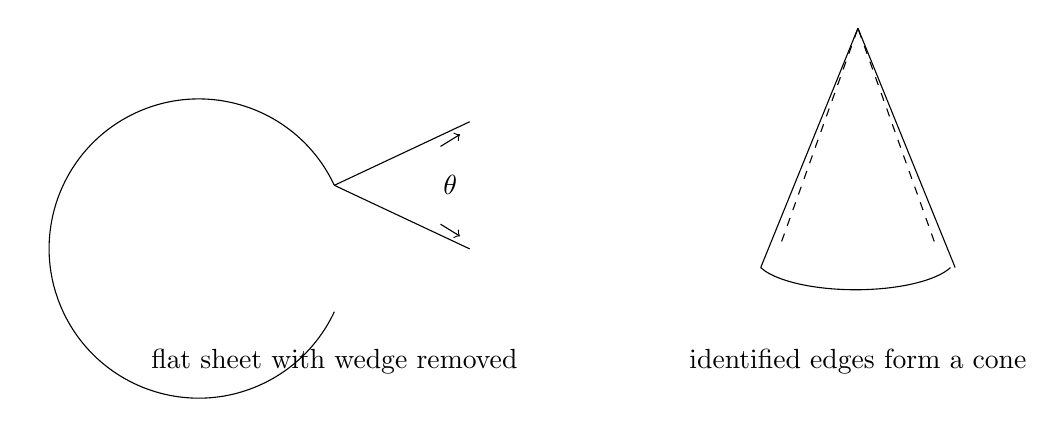
\begin{tikzpicture}[scale=0.95]
\draw (-4.2,0) arc[start angle=25,end angle=335,radius=2.0];
\draw (-4.2,0) -- (-2.39,0.85);
\draw (-4.2,0) -- (-2.39,-0.85);
\draw[->] (-2.78,0.52) -- (-2.52,0.68);
\draw[->] (-2.78,-0.52) -- (-2.52,-0.68);
\node at (-2.65,0.0) {$\theta$};
\node at (-4.2,-2.35) {flat sheet with wedge removed};

\draw (2.8,2.1) -- (1.5,-1.1);
\draw (2.8,2.1) -- (4.1,-1.1);
\draw (1.5,-1.1) arc[start angle=200,end angle=340,x radius=1.35,y radius=0.45];
\draw[dashed] (1.78,-0.75) -- (2.8,2.1);
\draw[dashed] (3.82,-0.75) -- (2.8,2.1);
\node at (2.8,-2.35) {identified edges form a cone};
\end{tikzpicture}
\caption{The cone as a flat sheet with an angular deficit and the corresponding identified surface.}
\end{figure}

The cone is produced by cutting an angular wedge out of a flat sheet and identifying the cut edges. Away from the tip the geometry is flat. Only the tip is special. The lecture uses this in exactly the right way: first to show how curvature may be concentrated at a point, then to show what parallel transport actually detects.

\begin{figure}[h]
\centering
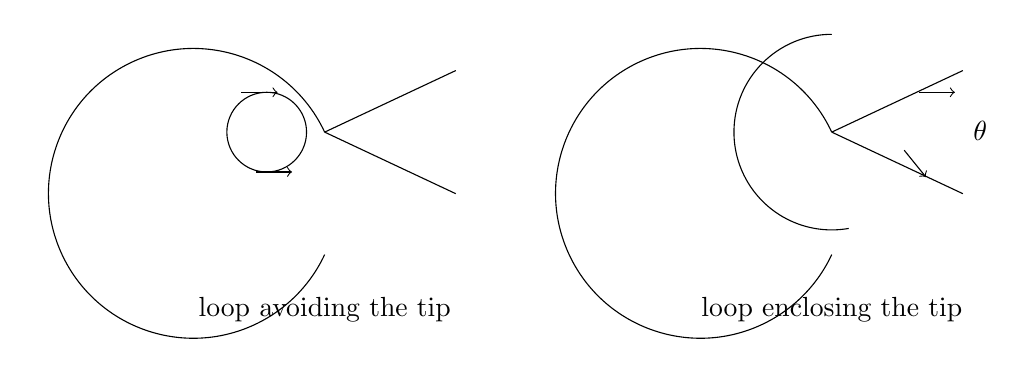
\begin{tikzpicture}[scale=0.92]
\draw (-4.0,0) arc[start angle=25,end angle=335,radius=2.0];
\draw (-4.0,0) -- (-2.19,0.85);
\draw (-4.0,0) -- (-2.19,-0.85);
\draw (-4.8,0.0) circle (0.55);
\draw[->] (-5.15,0.55) -- (-4.65,0.55);
\draw[->] (-4.95,-0.55) -- (-4.45,-0.55);
\node at (-4.0,-2.45) {loop avoiding the tip};

\draw (3.0,0) arc[start angle=25,end angle=335,radius=2.0];
\draw (3.0,0) -- (4.81,0.85);
\draw (3.0,0) -- (4.81,-0.85);
\draw (3.0,1.35) arc[start angle=90,end angle=280,radius=1.35];
\draw[->] (4.20,0.55) -- (4.70,0.55);
\draw[->] (4.00,-0.25) -- (4.30,-0.62);
\node at (5.05,0.02) {$\theta$};
\node at (3.0,-2.45) {loop enclosing the tip};
\end{tikzpicture}
\caption{A loop that avoids the cone tip returns the vector unchanged; a loop that encloses the tip returns it rotated by the angular deficit.}
\end{figure}

If the loop stays away from the tip, the relevant region can be opened out onto the flat sheet, and the transported vector comes back to itself. But if the loop encloses the tip, the identification of the cut edges forces a mismatch. The vector comes back rotated by the angular deficit:
\begin{equation}
\Delta\theta=\theta.
\end{equation}
The striking feature is that the detailed shape of the loop does not matter. What matters is whether the loop winds around the tip. The same point of curvature rotates the vector by the same amount.

The lecture then sharpens the example. Suppose we smooth off the cone tip instead of leaving it singular. A large loop around the same region will still detect curvature inside. So the closed-loop test locates the presence of curvature in the interior, but not necessarily its detailed distribution. On the sharp cone the curvature is concentrated at a single point. On the smoothed cone it is spread over a small cap. The loop knows there is curvature in there; it does not yet know precisely how it is distributed.

There is another benefit to the cone. It lets us think about geodesics by cutting and pasting. In the opened flat picture, geodesics are just straight lines. If a line crosses the cut, we simply re-open the cone elsewhere so that the same intrinsic geodesic is represented by a straight line on the new flat chart. This is the lecture's preferred way to think about geodesics on the cone: not by forcing them into the original slit representation, but by moving the slit until the straightness becomes visible.

The sphere supplies the smooth version of the same idea. Take a small loop on a sphere. The lecture asks us to imagine a cone tangent to the sphere all along that loop. A tiny creature living on the surface and carrying a little gyroscope cannot distinguish, by purely local measurements along the loop, whether it lives on the sphere or on that tangent cone. Therefore the transported vector undergoes the same net rotation in both cases.

\begin{figure}[h]
\centering
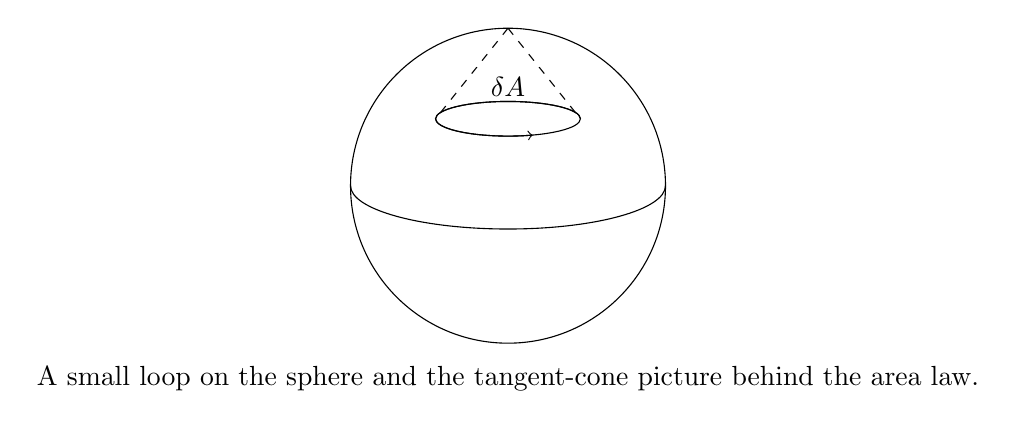
\begin{tikzpicture}[scale=1.0]
\draw (0,0) circle (2.0);
\draw (-2.0,0) arc[start angle=180,end angle=360,x radius=2.0,y radius=0.55];
\draw[dashed] (0,2.0) -- (-0.92,0.85);
\draw[dashed] (0,2.0) -- (0.92,0.85);
\draw (0,0.85) ellipse (0.92 and 0.22);
\draw[->] (0.92,0.85) arc[start angle=0,end angle=290,x radius=0.92,y radius=0.22];
\node at (0,1.25) {$\delta A$};
\node at (0,-2.45) {A small loop on the sphere and the tangent-cone picture behind the area law.};
\end{tikzpicture}
\caption{For a sufficiently small loop on a smooth surface, the transport defect is controlled by the enclosed area.}
\end{figure}

For small loops the rotation is small, and the lecture states the local two-dimensional law
\begin{equation}
\delta\theta \propto \delta A.
\end{equation}
More precisely, one defines the local curvature \(R\) by
\begin{equation}
\delta\theta=R\,\delta A
\end{equation}
for an infinitesimal loop. This is not yet the general curvature tensor of four-dimensional space-time. It is the local curvature law for a two-dimensional surface. It says that curvature measures the infinitesimal rate at which parallel transport around a tiny loop rotates a vector.

The lecture is careful about the domain of this formula. It is a small-loop statement. For large loops one needs the full integral effect, not merely the infinitesimal coefficient. That is why the formula should be read as local.

\subsection{Question \& Answer}

\paragraph{Do the transported vectors have to lie in the surface, and is parallel transport just keeping them parallel in the embedding space?}

No on both counts, at least not in the naive sense. On a two-dimensional surface the vector is best thought of as an element of the tangent space at each point. It points along the surface, but it is not literally a little stick glued into some ambient three-dimensional space. That is why parallel transport is an intrinsic notion. It is not defined by keeping the vector parallel in the larger embedding space and then projecting back. If one did that, the whole intrinsic notion of curvature would be lost. The lecture returns to this point near the end: intrinsic parallel transport lives in the tangent spaces of the geometry itself.

The lecture next introduces the sign of curvature. Give the enclosed area a sign by orienting the boundary of the loop. If we traverse the loop counterclockwise, say, we call the area positive; the opposite orientation is negative. Positive curvature means that the transported vector rotates in the same sense as the oriented loop, while negative curvature means it rotates in the opposite sense:
\begin{equation}
\operatorname{sign}(\delta\theta)=\operatorname{sign}(\delta A)
\qquad \text{for positive curvature.}
\end{equation}

\begin{figure}[h]
\centering
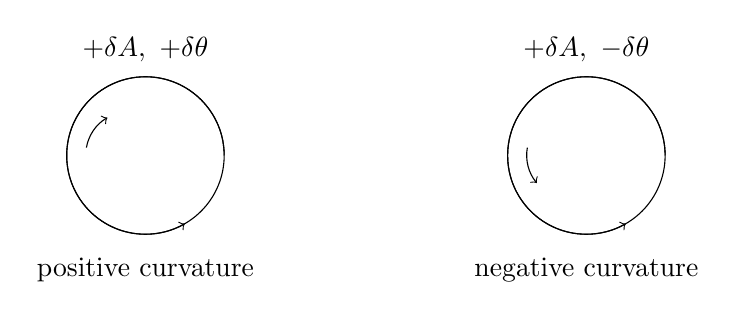
\begin{tikzpicture}[scale=1.0]
\draw (-2.8,0) circle (1.0);
\draw[->] (-1.8,0) arc[start angle=0,end angle=300,radius=1.0];
\draw[->] (-3.55,0.10) arc[start angle=170,end angle=120,radius=0.55];
\node at (-2.8,1.35) {$+\delta A,\ +\delta\theta$};
\node at (-2.8,-1.45) {positive curvature};

\draw (2.8,0) circle (1.0);
\draw[->] (3.8,0) arc[start angle=0,end angle=300,radius=1.0];
\draw[->] (2.05,0.10) arc[start angle=170,end angle=220,radius=0.55];
\node at (2.8,1.35) {$+\delta A,\ -\delta\theta$};
\node at (2.8,-1.45) {negative curvature};
\end{tikzpicture}
\caption{For an oriented loop, positive curvature rotates the transported vector in the same sense as the loop, while negative curvature rotates it in the opposite sense.}
\end{figure}

The sphere is the model of positive curvature. A saddle surface is the model of negative curvature. The lecture even gives a cut-and-paste version of negative curvature: instead of removing a wedge, insert an extra wedge. Then a counterclockwise circuit makes the vector rotate clockwise. The inner region of an ordinary torus is of this saddle type, while the outer region is sphere-like and positively curved. The torus is therefore useful as a mixed example: positive curvature outside, negative curvature inside. The Mobius strip is mentioned as a global oddity, but the lecture clearly treats it as a side remark rather than part of the main mathematical spine.

Finally the discussion lifts back to space-time. The words are the same, even if the visualization is not. There are curves in space-time, there is parallel transport, and the failure of a vector to return to itself around a closed loop is still the sign of curvature. The real gravitational field is precisely this space-time curvature, not merely the effect of funny coordinates. Mass, and more generally energy and momentum, create curvature. Particles then move on geodesics of the curved space-time. In the appropriate limit those geodesics reproduce Newtonian motion, with small relativistic corrections.

That is where the lecture stops. The next step, deferred to the following lecture, is to convert this geometric picture into the curvature tensor itself.

\section{Summary}

The lecture does not begin with curvature tensors or field equations. It begins more patiently: with the space-time interval, proper time, and the Minkowski signature. From there it separates curved coordinates from genuine curvature by way of the accelerated elevator and tidal forces. Flatness is then defined as the ability to choose coordinates in which the metric is constant, or equivalently has vanishing first derivatives. At a single point this can always be done, and the Christoffel symbols can be made to vanish there as well. That local flattening is the mathematical form of the free-fall principle.

Only after that does the lecture return to curves. The tangent vector gives the geodesic equation, and the more general condition \(D v^{m}/Ds=0\) defines parallel transport for any vector along any curve. The central test for curvature is then path dependence: transport a vector around a closed loop and see whether it comes back unchanged. The cone gives the sharp example, the sphere the smooth one, and the small-loop law \(\delta\theta=R\,\delta A\) gives the local two-dimensional measure.

The final physical point is the one general relativity needs. Space-time curvature is the genuine gravitational field. Energy and momentum create that curvature, and particles move on the resulting geodesics. The next lecture will give that idea its tensorial form.